\begin{frame}{Konstrukcija pravokotnice}
	
	\begin{columns}
		\begin{column}{0.55\textwidth}
			\begin{itemize}[<+->]
				\item Dana sta premica \(p\) in točka \(T\).
				\item Nariši lok \(k\) s središčem v \(T\).
				\item Lok \(k\) seče premico \(p\) v točkah \(A\) in \(B\).
				\item Nariši lok \(m\) s središčem v \(A\).
				\item Nariši lok \(n\) s središčem v \(B\) in z enakim polmerom.
				\item Loka se sečeta v točki \(C\).
				\item Premica \(TC\) je pravokotna na \(p\).
			\end{itemize}
		\end{column}
	
		\begin{column}{0.45\textwidth}
			\only<1>{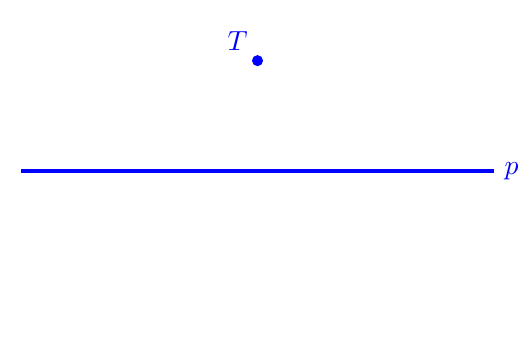
\includegraphics[width=50mm]{slike/fig-1.png}
			\centering}%
			\only<2>{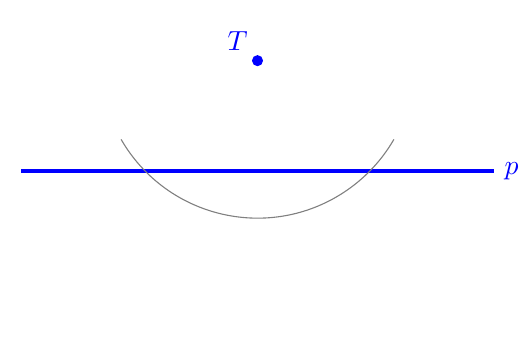
\includegraphics[width=50mm]{slike/fig-2.png}
			\centering}%
			\only<3>{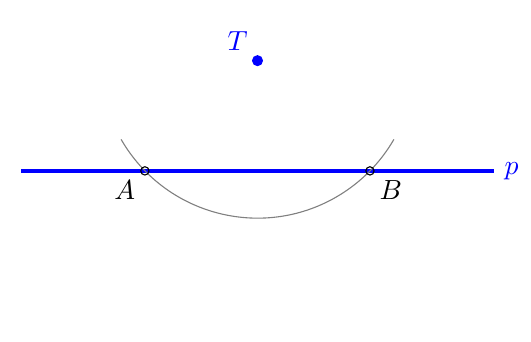
\includegraphics[width=50mm]{slike/fig-3.png}
			\centering}%
			\only<4>{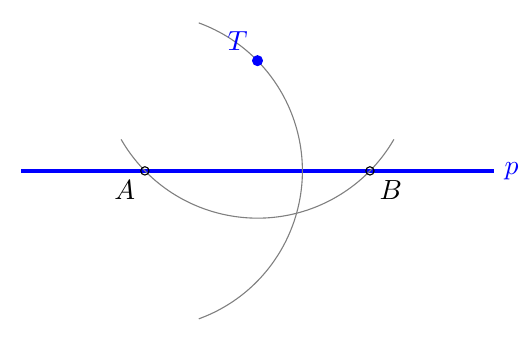
\includegraphics[width=50mm]{slike/fig-4.png}
			\centering}%
			\only<5>{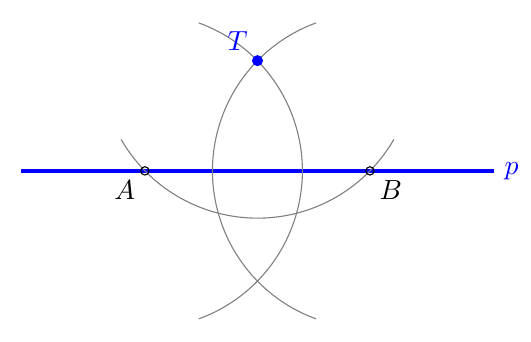
\includegraphics[width=50mm]{slike/fig-5.png}
			\centering}%
			\only<6>{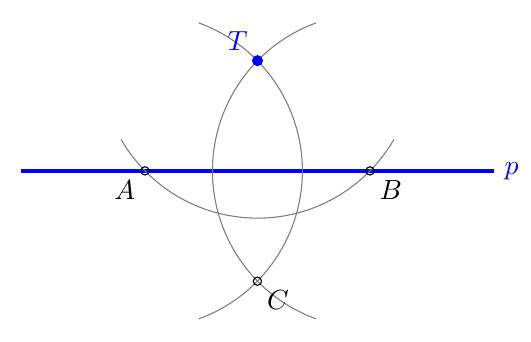
\includegraphics[width=50mm]{slike/fig-6.png}
			\centering}%
			\only<7>{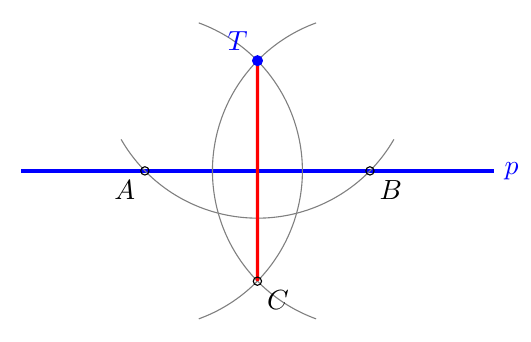
\includegraphics[width=50mm]{slike/fig-7.png}
			\centering}%
		\end{column}
	\end{columns}
\end{frame}
